% !Mode:: "TeX:UTF-8:Main"
% gif command (hope it still works ...)
% magick -density 160 -delay 35 -loop 0 XXXX.pdf XXXX.gif

\documentclass{beamer}
\usepackage[T1]{fontenc}
\setbeamertemplate{navigation symbols}{}
\usepackage{tikzducks,tikzlings}
\usepackage{fontawesome}

\usetikzlibrary{positioning,calc}

\setbeamercolor{background canvas}{bg=white!20!black}

\begin{document}

\begin{frame}
\vspace*{.5ex}
\begin{tikzpicture}
\node[draw, fill=black, rectangle, minimum width=2.5cm, minimum height=1.5cm, rounded corners, align=center, text width=2cm] (cam1) {\color{white}\bfseries\small Dürer, the rhino};

\node at ([yshift=-.25cm, xshift=-.2cm]cam1.north east) {\color{white}\bfseries\tiny\faMicrophoneSlash};

\node[draw, fill=white!50!black, rectangle, minimum width=2.5cm, minimum height=1.5cm, rounded corners, right=.2cm of cam1] (cam2) {};

\begin{scope} 
  \clip (cam2.south west) rectangle (cam2.north east);
  \bear[yshift=-1.5cm, xshift=2.65cm]
\end{scope}

\node [draw, rectangle, fill=black, rounded corners=2pt, inner sep=2pt, minimum width=2.3cm] at ([yshift=0cm]cam2.south) {\color{white}\bfseries\tiny Bär, the teddy bear};

\node at ([yshift=-.25cm, xshift=-.2cm]cam2.north east) {\bfseries\tiny\faMicrophoneSlash};

\node[draw, fill=white!50!black, rectangle, minimum width=2.5cm, minimum height=1.5cm, rounded corners, right=.2cm of cam2] (cam3) {};

\begin{scope} 
  \clip (cam3.south west) rectangle (cam3.north east);
  \squirrel[yshift=-1.5cm, xshift=5.2cm]
\end{scope}

\node [draw, rectangle, fill=black, rounded corners=2pt, inner sep=2pt, minimum width=2.3cm] at ([yshift=0cm]cam3.south) {\color{white}\bfseries\tiny Ratatosk, the squirrel};

\node at ([yshift=-.25cm, xshift=-.2cm]cam3.north east) {\bfseries\tiny\faMicrophoneSlash};

\node[draw, fill=white!50!black, rectangle, minimum width=2.5cm, minimum height=1.5cm, rounded corners, right=.2cm of cam3] (cam4) {};

\begin{scope} 
  \clip (cam4.south west) rectangle (cam4.north east);
  \coati[yshift=-1.65cm, xshift=8cm]
\end{scope}

\node [draw, rectangle, fill=black, rounded corners=2pt, inner sep=2pt, minimum width=2.3cm] at ([yshift=0cm]cam4.south) {\color{white}\bfseries\tiny 007, the coati};

\node at ([yshift=-.25cm, xshift=-.2cm]cam4.north east) {\bfseries\tiny\faMicrophoneSlash};

\node[draw, fill=white!50!black, rectangle, minimum width=2.5cm, minimum height=1.5cm, rounded corners, below=.2cm of cam4] (cam5) {};

\begin{scope} 
  \clip (cam5.south west) rectangle (cam5.north east);
  \koala[yshift=-3.5cm, xshift=8.2cm]
\end{scope}

\node [draw, rectangle, fill=black, rounded corners=2pt, inner sep=2pt, minimum width=2.3cm] at ([yshift=0cm]cam5.south) {\color{white}\bfseries\tiny Will, the koala};

\node at ([yshift=-.25cm, xshift=-.2cm]cam5.north east) {\bfseries\tiny\faMicrophone};

\node[draw, fill=white!50!black, rectangle, minimum width=2.5cm, minimum height=1.5cm, rounded corners, below=.2cm of cam5] (cam6) {};

\begin{scope} 
  \clip (cam6.south west) rectangle (cam6.north east);
  \mouse[yshift=-5.2cm, xshift=8.2cm]
\end{scope}

\node [draw, rectangle, fill=black, rounded corners=2pt, inner sep=2pt, minimum width=2.3cm] at ([yshift=0cm]cam6.south) {\color{white}\bfseries\tiny Tokz, the mouse};

\node at ([yshift=-.25cm, xshift=-.2cm]cam6.north east) {\bfseries\tiny\faMicrophoneSlash};

\node[draw, fill=white!50!black, rectangle, minimum width=2.5cm, minimum height=1.5cm, rounded corners, below=.2cm of cam6] (cam7) {};

\begin{scope} 
  \clip (cam7.south west) rectangle (cam7.north east);
  \owl[yshift=-6.8cm, xshift=8.2cm]
\end{scope}

\node [draw, rectangle, fill=black, rounded corners=2pt, inner sep=2pt, minimum width=2.3cm] at ([yshift=0cm]cam7.south) {\color{white}\bfseries\tiny Jake, the owl};

\node at ([yshift=-.25cm, xshift=-.2cm]cam7.north east) {\bfseries\tiny\faMicrophoneSlash};

\node[draw, fill=white!50!black, rectangle, minimum width=2.5cm, minimum height=1.5cm, rounded corners, below=.2cm of cam7] (cam8) {};

\begin{scope} 
  \clip (cam8.south west) rectangle (cam8.north east);
  \pig[yshift=-8.6cm, xshift=8.2cm]
\end{scope}

\node [draw, rectangle, fill=black, rounded corners=2pt, inner sep=2pt, minimum width=2.3cm] at ([yshift=0cm]cam8.south) {\color{white}\bfseries\tiny Ms Piggy, the pig};

\node at ([yshift=-.25cm, xshift=-.2cm]cam8.north east) {\bfseries\tiny\faMicrophoneSlash};

\node[draw, fill=white!50!black, rectangle, minimum width=7.9cm, minimum height=5.5cm, rounded corners, below=1cm of cam1.east, xshift=1.45cm] (cam9) {};

\begin{scope} 
  \clip (cam9.south west) rectangle (cam9.north east);
  \anteater[yshift=-9.1cm, xshift=1.9cm, scale=3.5]
\end{scope}

\node [draw, rectangle, fill=black, rounded corners=2pt, inner sep=2pt, minimum width=7.7cm] at ([yshift=0cm]cam9.south) {\color{white}\bfseries\tiny Peter, the anteater};

\node[draw, fill=white!80!black, rectangle, minimum width=10.6cm, minimum height=.5cm, rounded corners, above=1cm of cam1.east, xshift=2.8cm] (titlebar) {\bfseries\ \faAlignJustify\ TikZlings meeting -- Zoom};

\node[draw, fill=white!80!black, circle, minimum width=.66cm, below=.4cm of cam9, inner sep=0pt] (icon1) {\faVideoCamera};
\node[draw, fill=white!80!black, circle, minimum width=.66cm, left=.2cm of icon1, inner sep=0pt] (icon2) {\faMicrophoneSlash};
\node[draw, fill=white!80!black, circle, minimum width=.66cm, right=.2cm of icon1, inner sep=0pt] (icon3) {\faVolumeUp};
\end{tikzpicture}
\end{frame}
\end{document}
